\item \textbf{Problem 1.11}
Construct $\ket{\vb S\cdot\vu n;+}$ such that
\[
\vb S \cdot \vu n \ket{\vb S\cdot\vu n;+} = \qty(\frac{\hbar}{2}) \ket{\vb S\cdot\vu n;+}
\]
where $\vu n$ is characterized by the angles shown in the figure. Express your answer as a
linear combination of $\ket+$ and $\ket -$. [Note: The answer is
\[
\cos(\frac \beta2) \ket + \sin(\frac \beta2) e^{i\alpha}\ket -.
\]
\begin{figure}[h]
    \centering
    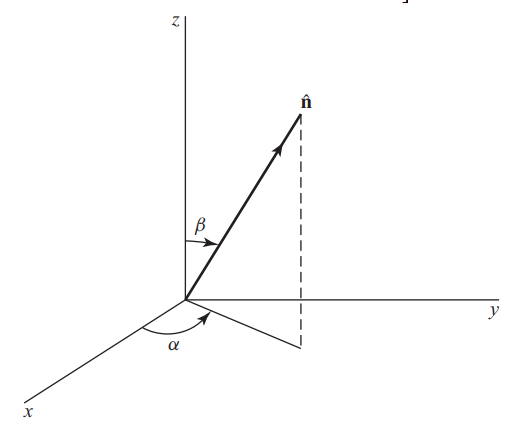
\includegraphics[width=0.5\linewidth]{P4.png}
\end{figure}

\textbf{Solution}

We begin by writing the matrix representation of this eigenvalue problem and then solving the eigenvalue problem stated above with the given eigenvalue $\frac{\hbar}{2}$ to find the eigenvector.

\begin{gather*}
\vb S \cdot \vu n = S_x \sin\beta \cos\alpha + S_y \sin\beta\sin\alpha + S_z \cos\beta\\
=\frac\hbar2 \mqty(\cos\beta & \sin\beta\cos\alpha - i\sin\beta\sin\alpha\\
                \sin\beta\cos\alpha + i\sin\beta\sin\alpha & -\cos\beta) = \frac\hbar2 \mqty(\cos\beta & \sin\beta e^{-i\alpha} \\ \sin\beta e^{i\alpha} & -\cos\beta)\\
\end{gather*}
We use this matrix and solve the eigenvalue equation
\begin{gather*}
    (\vb S\cdot \vu n - \frac\hbar2 \mathbb{I}) X = 0\\
    \frac{\hbar}{2} \mqty(\cos\beta -1 & \sin\beta e^{-i\alpha} \\ \sin\beta e^{i\alpha} & -\cos\beta - 1) \mqty(x \\ y) = \mqty(0\\0)\\
\end{gather*}
This gives us 2 equations

\begin{gather}
    (\cos\beta - 1)x + (\sin\beta e^{-i\alpha})y = 0\\
     (\sin\beta e^{i\alpha})x -(\cos\beta + 1)y = 0
\end{gather}
     From equation (2) we get the expression
     \[
     y= \frac{\sin\beta e^{i\alpha}}{\cos\beta+1} x
     \]

     And so our eigenvector can be written as
     \begin{gather*}
         \mqty[1 \\ \frac{\sin\beta e^{i\alpha}}{\cos\beta+1}] = \mqty[ 1 \\ \frac{\sin\beta e^{i\alpha}}{2\cos[2](\beta/2)}] = \mqty[\cos(\beta/2)\\ \frac{\sin\beta e^{i\alpha}}{2\cos(\beta/2)} ] = \mqty[  \cos\frac\beta2\\ \sin\frac\beta2 e^{i\alpha}  ]
     \end{gather*}

     Where I have used the relations
     \begin{align*}
         \cos\beta + 1 = 2\cos[2](\frac{\beta}{2}) && \sin\beta = 2\sin(\frac\beta2) \cos(\frac\beta2)
     \end{align*}
     and so using $x \to \ket +$ and $y \to \ket -$ we have

\[
\ket{\vb S\cdot\vu n;+} = \cos(\frac\beta2) \ket + + \sin(\frac\beta2)e^{i\alpha}
\]
